\documentclass{article}
\usepackage{hyphenat}

% if you need to pass options to natbib, use, e.g.:
%     \PassOptionsToPackage{numbers, compress}{natbib}
% before loading neurips_2026
\PassOptionsToPackage{numbers,compress}{natbib}

% The authors should use one of these tracks.
% Before accepting by the NeurIPS conference, select one of the options below.
% 0. "default" for submission
\usepackage[main, final]{neurips_2026}
% the "default" option is equal to the "main" option, which is used for the Main Track with double-blind reviewing.
% 1. "main" option is used for the Main Track
%  \usepackage[main]{neurips_2026}
% 2. "position" option is used for the Position Paper Track
%  \usepackage[position]{neurips_2026}
% 3. "eandd" option is used for the Evaluations & Datasets Track
 % \usepackage[eandd]{neurips_2026}
% 4. "creativeai" option is used for the Creative AI Track
%  \usepackage[creativeai]{neurips_2026}
% 5. "sglblindworkshop" option is used for the Workshop with single-blind reviewing
 % \usepackage[sglblindworkshop]{neurips_2026}
% 6. "dblblindworkshop" option is used for the Workshop with double-blind reviewing
%  \usepackage[dblblindworkshop]{neurips_2026}

% After being accepted, the authors should add "final" behind the track to compile a camera-ready version.
% 1. Main Track
 % \usepackage[main, final]{neurips_2026}
% 2. Position Paper Track
%  \usepackage[position, final]{neurips_2026}
% 3. Evaluations & Datasets Track
 % \usepackage[eandd, final]{neurips_2026}
% 4. Creative AI Track
%  \usepackage[creativeai, final]{neurips_2026}
% 5. Workshop with single-blind reviewing
%  \usepackage[sglblindworkshop, final]{neurips_2026}
% 6. Workshop with double-blind reviewing
%  \usepackage[dblblindworkshop, final]{neurips_2026}
% Note. For the workshop paper template, both \title{} and \workshoptitle{} are required, with the former indicating the paper title shown in the title and the latter indicating the workshop title displayed in the footnote.
% For workshops (5., 6.), the authors should add the name of the workshop, "\workshoptitle" command is used to set the workshop title.
% \workshoptitle{WORKSHOP TITLE}

% "preprint" option is used for arXiv or other preprint submissions
 % \usepackage[preprint]{neurips_2026}

% to avoid loading the natbib package, add option nonatbib:
%    \usepackage[nonatbib]{neurips_2026}

\usepackage[utf8]{inputenc} % allow utf-8 input
\usepackage[T1]{fontenc}    % use 8-bit T1 fonts
\usepackage{hyperref}       % hyperlinks
\usepackage{url}            % simple URL typesetting
\usepackage{booktabs}       % professional-quality tables
\usepackage{amsfonts}       % blackboard math symbols
\usepackage{nicefrac}       % compact symbols for 1/2, etc.
\usepackage{microtype}      % microtypography
\usepackage{xcolor}         % colors
\usepackage{graphicx}       % figures
\usepackage{caption}
\usepackage{natbib}
\usepackage{placeins}

% Update the title below with your final project title.
\title{Deep Learning for PJM Day-Ahead Electricity Price Forecasting}

% Put your group Canvas number and member names on the first page.
% You can replace the placeholders below with the exact names and section/group number.
\author{%
  Canvas Group Number: 25 
  \AND
  Allie Zong \And 
  Anthony Shen \And
  Lewis Tu \And
  Sam Chung
}

\begin{document}

\maketitle
\begin{abstract}
We forecast hourly PJM-RTO day-ahead electricity prices using leakage-safe features available before the day-ahead market clears. The unit of prediction is an hourly price in \$/MWh, evaluated on a chronological held-out test set. Using PJM price, load forecast, generation, outage, and calendar data, we compare persistence baselines, Random Forest, and an LSTM sequence model. The final LSTM achieves a test MAE of 7.69 and RMSE of 13.86, improving over the 48-hour persistence baseline by 47.8\% in MAE and 41.5\% in RMSE. However, the Random Forest attains a slightly lower RMSE, so the strongest conclusion is that leakage-safe machine learning improves over naive persistence, not that LSTMs dominate all alternatives.
\end{abstract}

\section{Background \& Motivation}

PJM Interconnection operates the high-voltage grid and wholesale electricity markets for all or part of 13 states and the District of Columbia, serving more than 67 million people \cite{pjm_who_we_are,ferc_pjm}. Its energy market includes both a Day-Ahead Market, which schedules electricity one day before delivery, and a Real-Time Market, which balances conditions during the operating day at five-minute intervals \cite{pjm_energy_market}. In the Day-Ahead Market, hourly clearing prices are determined for the next operating day from submitted supply offers, demand bids, and related transactions \cite{pjm_manual11}.

Forecasting day-ahead prices is difficult because electricity demand and supply conditions can shift quickly. Weather-driven load changes, generation outages, fuel-cost changes, and renewable generation variability can all affect market outcomes. When day-ahead expectations differ from actual operating conditions, the Real-Time Market helps correct the imbalance, often under tighter operational constraints. For this reason, better day-ahead price forecasts can support more informed decisions before electricity is delivered.

This project matters because PJM day-ahead prices affect multiple decision makers. Generators can use forecasts to inform bidding, fuel procurement, and unit-commitment decisions. Utilities, load-serving entities, and large consumers can use them for budgeting, hedging, and demand-response planning. Our work therefore supports a decision-support setting: estimating next-day hourly prices early enough to inform market and operational planning, while recognizing that forecasts cannot eliminate uncertainty in volatile electricity markets.

\section{Problem Statement}

We ask whether historical PJM day-ahead price data, lagged system variables, and calendar features available before the day-ahead market clears can be used to predict hourly PJM day-ahead electricity prices for the next operating day more accurately than persistence baselines.

\begin{itemize}
  \item \textbf{Target/output:} Hourly PJM day-ahead electricity prices, measured in \$/MWh, for the next operating day.
  
  \item \textbf{Unit of observation:} One PJM operating day. Each observation is a 24-hour regional price profile, with one predicted price for each delivery hour.
  
  \item \textbf{Prediction setting:} Forecasts are made before the day-ahead market clears at 10:30 AM on the prior day. The model uses only information assumed to be available by that cutoff, including historical prices, lagged market and system variables, and calendar features.
  
  \item \textbf{Success metric:} We evaluate performance using MAE and RMSE, comparing neural-network models against persistence baselines. MAE summarizes typical hourly error, while RMSE places more weight on large misses during volatile price periods.
\end{itemize}

\section{Data \& Exploratory Data Analysis}

\subsection{Data sources and preprocessing}

We model hourly PJM-RTO day-ahead electricity prices using a merged hourly dataset constructed from PJM Data Miner 2 files. The target is PJM-RTO day-ahead locational marginal price, using \texttt{pnode\_id = 1} and renaming \texttt{total\_lmp\_da} as \texttt{price}. We merge this target with RTO load forecasts, generation by fuel type, and forecasted generation outages. All sources are aligned by Eastern Prevailing Time using hourly timestamps. The resulting reusable feature table, \texttt{initial\_data.csv}, contains 8,736 hourly observations and 28 columns.

The preprocessing pipeline keeps the problem at the system-wide PJM-RTO level rather than modeling individual zones. Load forecasts are filtered to the aggregate RTO forecast area. Generation is pivoted into fuel-specific hourly columns, including coal, gas, nuclear, wind, solar, hydro, oil, storage, multiple fuels, and other renewables; renewable generation is also aggregated into \texttt{renewable\_mw}. Forecasted outages are merged at the RTO level. Calendar variables are added because they are known before the auction clears: hour, day of week, month, weekend indicator, holiday indicator, season, and cyclical sine/cosine encodings for hour and day of week.

A key preprocessing decision was to make the final feature set leakage-safe for the day-ahead setting. Because PJM day-ahead bids are assumed to be locked by 10:30 AM on day $D-1$ for delivery day $D$, the model should not use realized information from after that cutoff. We therefore use forecasted variables directly only when they are day-ahead forecasts, lag realized generation variables by 48 hours, and replace short-horizon price features with \texttt{price\_lag\_48}, \texttt{price\_lag\_168}, and a safe rolling 24-hour price feature computed only from prices available before the cutoff. 

\subsection{EDA findings that influenced modeling}

The EDA showed four patterns that directly shaped the models. First, day-ahead prices exhibit occasional large spikes over time, even though most hours remain near typical market levels. This spike behavior is visible in Figure~\ref{fig:eda-price-over-time}, where most of the series stays relatively low but several short periods show sharp upward movements. The raw price histogram, included in the appendix, further confirms that the target distribution is strongly right-skewed. This motivated reporting both MAE and RMSE: MAE better reflects typical-hour forecast error, while RMSE penalizes large spike-hour misses more heavily.

\begin{figure}[!htbp]
  \centering
  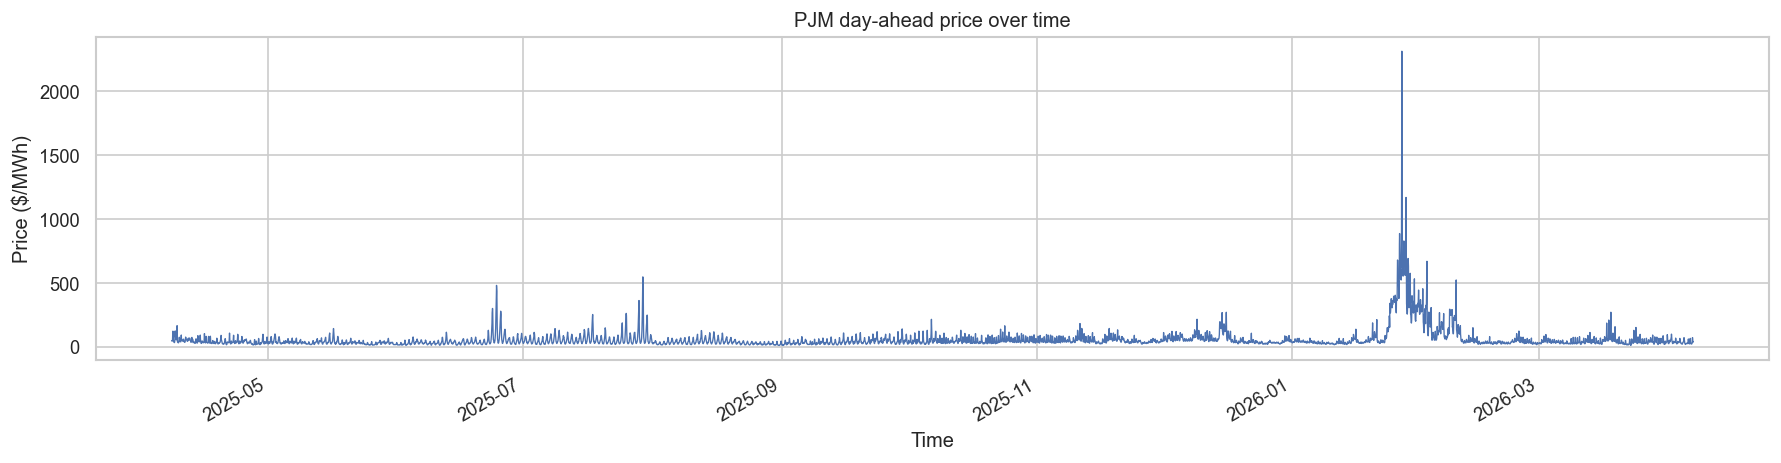
\includegraphics[width=0.85\linewidth]{../plots/eda_price_over_time.png}
  \caption{Target price over time}
  \label{fig:eda-price-over-time}
\end{figure}

Second, prices have clear calendar structure. Figure~\ref{fig:eda-average-hourly-price} shows morning and evening price peaks, while appendix plots show additional weekday/weekend, monthly, seasonal, and holiday differences. In particular, winter prices are noticeably higher, consistent with higher heating demand and tighter system conditions. These patterns justify including calendar variables and cyclical time encodings in the final models.

\begin{figure}[!htbp]
  \centering
  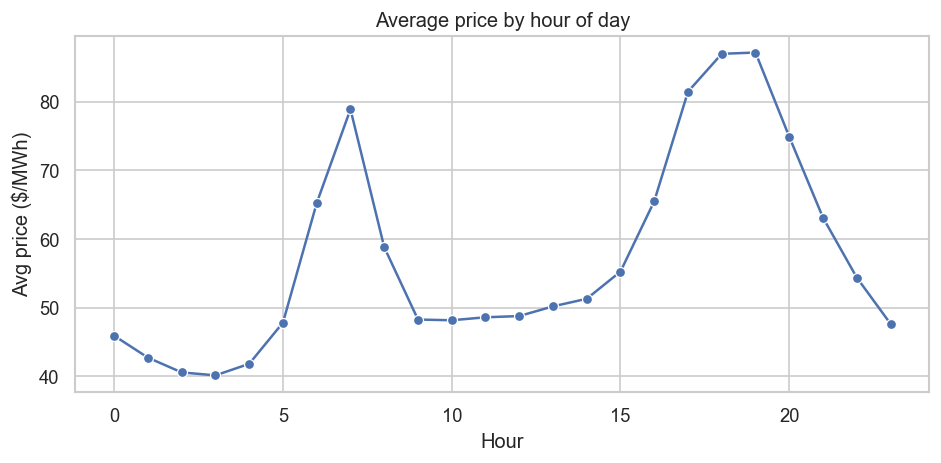
\includegraphics[width=0.72\linewidth]{../plots/eda_average_hourly_price.png}
  \caption{Average price by delivery hour}
  \label{fig:eda-average-hourly-price}
\end{figure}

Third, load forecast is one of the strongest exogenous signals. Figure~\ref{fig:price-vs-load-forecast} shows a visible positive relationship between \texttt{price} and \texttt{load\_forecast\_mw}, consistent with the supply-demand mechanism behind day-ahead electricity pricing. This supports keeping load forecast in the final  feature set rather than relying only on historical prices. This EDA result is later confirmed by permutation importance in the final model, where \texttt{load\_forecast\_mw} is the most important feature. 

\begin{figure}[!htbp]
  \centering
  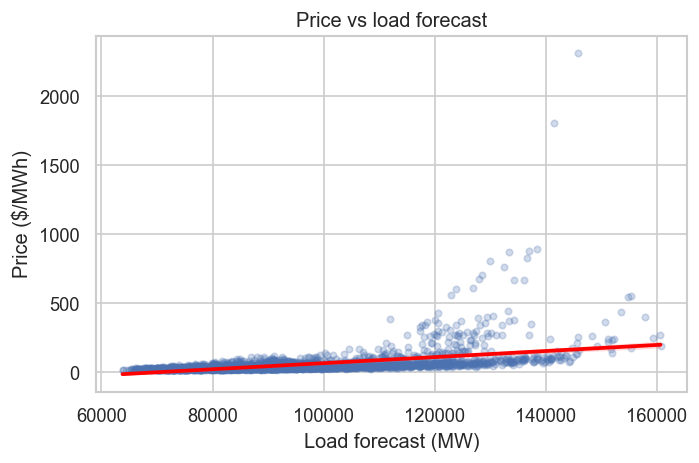
\includegraphics[width=0.72\linewidth]{../plots/eda_price_vs_load_forecast.png}
  \caption{Price and load forecast}
  \label{fig:price-vs-load-forecast}
\end{figure}

Fourth, the price series is highly persistent. Figure~\ref{fig:price-autocorrelation} shows that autocorrelation remains high across short horizons and displays daily structure around 24-hour multiples. The notebook also reports correlations of 0.946 between current price and \texttt{price\_lag\_1}, and 0.814 between current price and \texttt{price\_lag\_24}. Although those short lags are useful diagnostically, they are not fully consistent with the day-ahead information cutoff. This is why the final models use \texttt{price\_lag\_48} as the main persistence feature and \texttt{price\_lag\_168} to capture same-hour weekly seasonality. The same finding also motivates using persistence models as baselines: any useful machine learning model should beat a simple lag-based forecast.

\begin{figure}[!htbp]
  \centering
  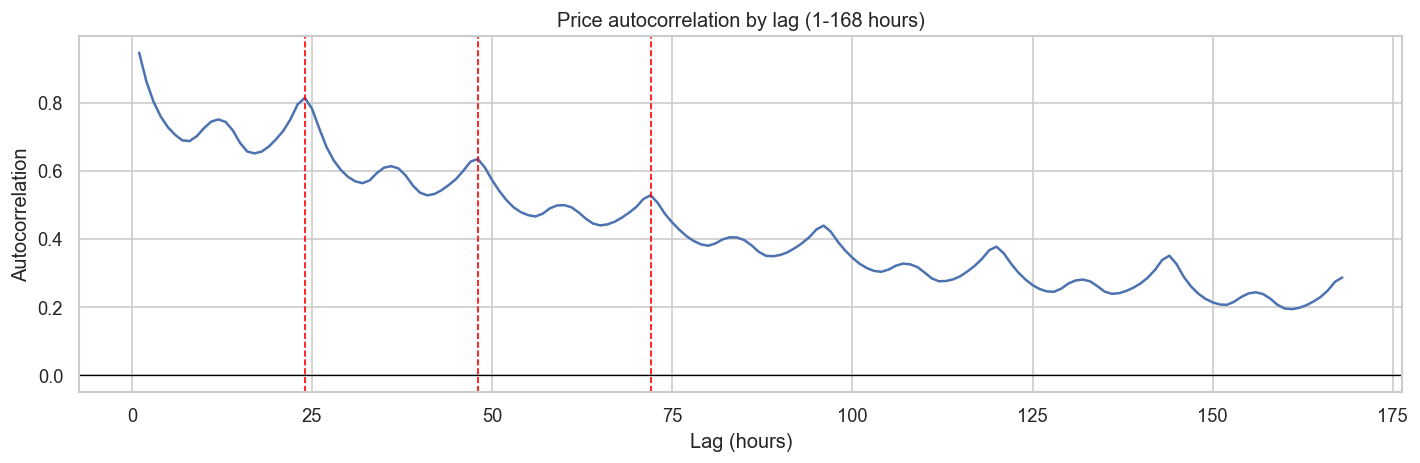
\includegraphics[width=1.0\linewidth]{../plots/eda_autocorrelation.png}
  \caption{Price autocorrelation}
  \label{fig:price-autocorrelation}
\end{figure}

Overall, the EDA narrowed the modeling problem to a leakage-safe hourly forecasting task with three main information sources: historical price persistence, known calendar structure, and day-ahead system conditions such as load forecasts and outage forecasts. This distilled feature design is used in the final LSTM and Random Forest comparisons rather than carrying forward every raw variable from the merged dataset.

\section{Methods \& Models}

\subsection{Baseline and model choices}

We replaced our earlier MS3 neural-network baseline with a leakage-safe persistence baseline because the MS3 models used short-horizon price features, including \texttt{price\_lag\_1}, \texttt{price\_lag\_24}, and an unsafe rolling price feature, which are not directly comparable to the final day-ahead setup. For the final report, the main baseline is a 48-hour persistence model:

\[
\hat{y}_t = y_{t-48}.
\]

This baseline predicts each hourly price using the price from two days earlier, which is consistent with the information available before the day-ahead market clears. We also checked a 168-hour weekly persistence baseline, but the 48-hour version performed better and is therefore the primary naive benchmark.

For machine learning models, we compared an LSTM sequence model with a Random Forest benchmark. We considered RNN, GRU, and LSTM architectures because hourly electricity prices are temporally ordered and recent history may help predict future prices. We selected the LSTM because its gated memory structure is better suited than a vanilla RNN for learning dependencies across hourly sequences. The Random Forest provides a strong non-sequential comparison, helping test whether performance gains come from sequence modeling or from the leakage-safe feature set itself.

\subsection{Final model pipeline}

The final LSTM predicts one hourly PJM-RTO day-ahead price at a time. All features were constructed to match the prediction setting: forecasts must be made before the PJM day-ahead market clears at 10:30 AM ET on day $D-1$ for delivery day $D$. To avoid leakage, we removed unsafe short-lag price features, lagged realized generation variables by 48 hours, and computed rolling price history only from prices available before the cutoff.

The final feature set includes four groups: leakage-safe price history, calendar and cyclical timing variables, day-ahead load and outage forecasts, and 48-hour-lagged generation by fuel type. Each LSTM input has shape

\[
(B, T, F),
\]

where $B$ is batch size, $T$ is the lookback window, and $F$ is the number of features. The selected lookback was $T=48$ hours, so each prediction uses the previous 48 hourly feature rows.

We used a strictly chronological train-validation-test split by delivery day, with no shuffling or k-fold cross-validation. This ensured that all 24 hours of each operating day stayed within one split and that the model was evaluated on future data only. Feature and target values were scaled using \texttt{StandardScaler} objects fit on the training set only, and predictions were inverse-transformed before computing MAE and RMSE.

Hyperparameters were selected using a small random search over lookback length, hidden size, number of layers, dropout, learning rate, and batch size. Each trial used Adam optimization, MSE loss, and early stopping on validation RMSE. The selected configuration used a 48-hour lookback, hidden size 128, one LSTM layer, dropout 0.3, learning rate \texttt{1e-3}, and batch size 32.

\FloatBarrier
\section{Results \& Interpretation}

Table~\ref{tab:model-results} compares the final LSTM with the persistence baseline and a Random Forest benchmark on the same chronological held-out test set. All metrics are reported in the original \$/MWh scale after inverse-transforming predictions.

\begin{table}[h]
  \caption{Model performance comparison on the held-out test set.}
  \label{tab:model-results}
  \centering
  \begin{tabular}{lccc}
    \toprule
    Model & MAE & RMSE & Notes \\
    \midrule
     Persistence 48h & 14.72 & 23.71 & Copies price from 48 hours earlier \\
    Random Forest & 8.04 & 13.26 & Strong non-sequential benchmark \\
    Final LSTM & 7.69 & 13.86 & Best average-error performance \\
    \bottomrule
  \end{tabular}
\end{table}

\subsection{Quantitative performance}

The final LSTM substantially improves over the 48-hour persistence baseline, reducing MAE from 14.72 to 7.69 and RMSE from 23.71 to 13.86. This corresponds to a 47.8\% reduction in MAE and a 41.5\% reduction in RMSE, showing that the model learns useful structure beyond simply copying a recent price. 

We also compared our LSTM performance against a Random Forest model on the same features. This comparison tests whether the added complexity of recurrent modeling improves performance for our forecasting task. The Random Forest model has slightly lower RMSE, while the LSTM has slightly lower MAE. This suggests that the LSTM performs better on typical hourly errors, while the Random Forest is somewhat better at limiting larger errors.

\begin{figure}
    \centering
    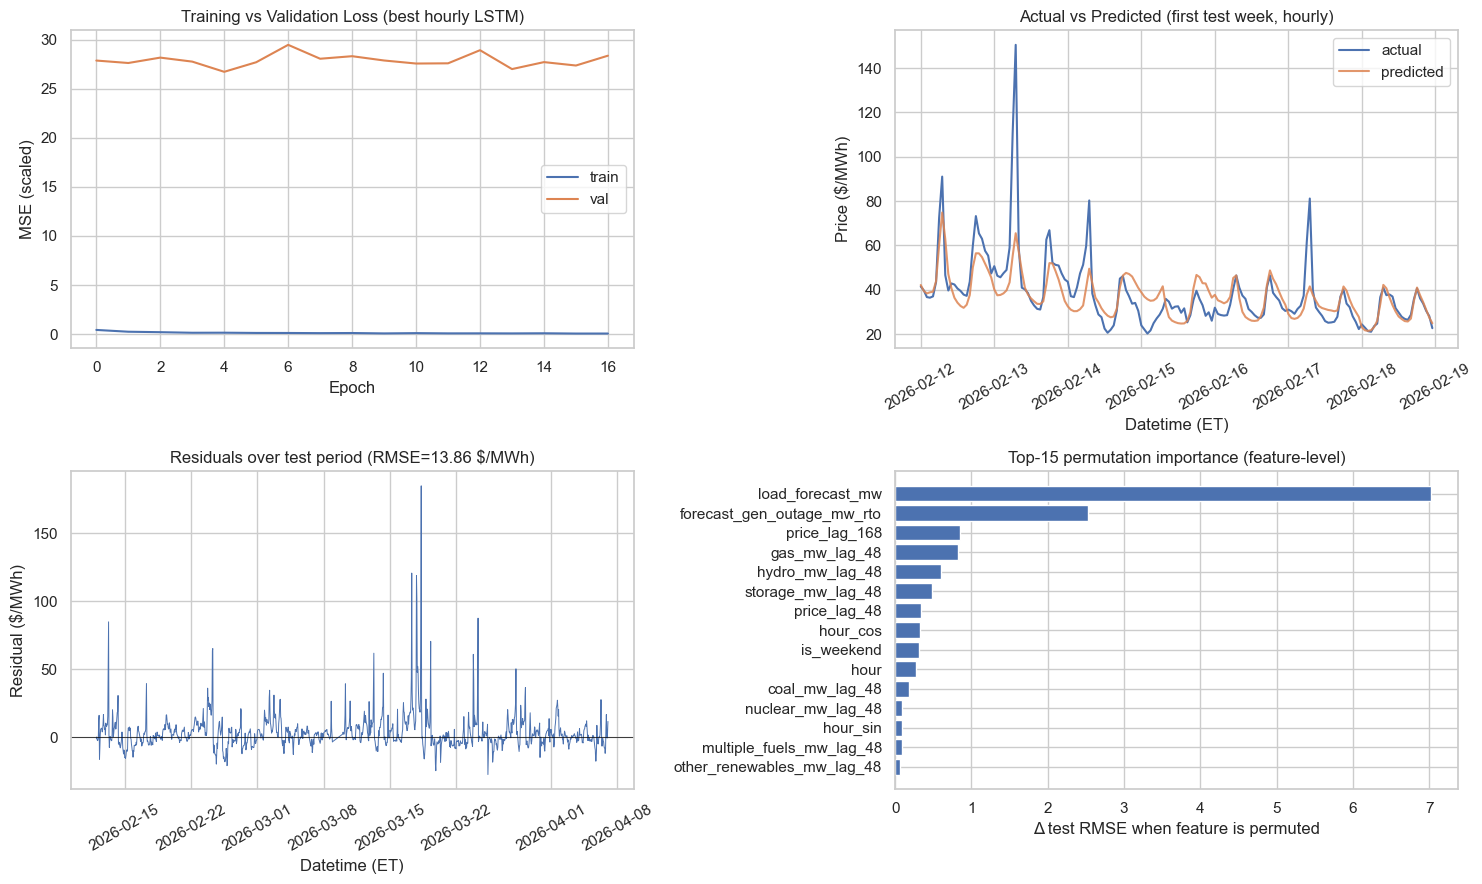
\includegraphics[width=0.9\linewidth]{../plots/5_2_1.png}
    \caption{Feature importance and prediction error patterns for the final LSTM}
    \label{fig:results-interpretation}
\end{figure}

\subsection{Model interpretation and error analysis}

Figure~\ref{fig:results-interpretation} summarizes the final model's training behavior, test predictions, residuals, and permutation importance.

Permutation importance shows that \texttt{load\_forecast\_mw} is the most important individual feature, followed by outage forecasts, price-history variables, and selected lagged generation variables. At the feature-group level, forecast features are most important, followed by lagged generation, price history, and calendar variables. This suggests that the model relies most on expected demand and supply conditions, while calendar variables mainly help capture repeated hourly and weekly patterns.

The model performs best on regular hourly price patterns but remains weaker during volatile periods and price spikes. This is reflected in the MAE/RMSE comparison: the LSTM's lower MAE suggests strong average-hour performance, while its RMSE remains affected by larger errors. The large gap between validation MSE and train/test MSE further suggests that the model struggled during the validation period, which coincided with a more volatile winter regime and likely included more peak-demand hours. Therefore, although the LSTM captures meaningful structure in PJM day-ahead prices, further testing across additional seasons and market conditions is needed before concluding that it generalizes reliably across the full PJM market.

\section{Conclusions \& Discussion}

Our project showed that by using machine learning techniques, we can meaningfully improve PJM day-ahead electricity price forecasting relative to a simple persistence baseline. The evidence supports using historical prices, load forecasts, outage forecasts, lagged generation mix, and calendar features when they are aligned to the day-ahead prediction setting. The final LSTM benefits from sequential structure, but much of the predictive signal comes from carefully timed features that reflect expected demand, supply constraints, and recent market behavior. However, the results do not show that LSTMs are clearly superior to all other models, since the Random Forest achieves a slightly lower RMSE.

The project has several limitations. The dataset covers roughly one year of system-wide PJM-RTO data, which limits exposure to different seasonal regimes and rare market events. The model also omits potentially important predictors such as weather, fuel prices, congestion, zonal price differences, bidding behavior, and plant-level constraints. These missing variables likely explain part of the remaining error, especially during price spikes. Finally, the LSTM produces point forecasts only, so it does not communicate uncertainty or explicitly flag high-risk spike periods.

\subsection{Future work}

Future work should expand the dataset beyond one year, add richer external features, and evaluate the model with rolling time-based validation. Weather forecasts, fuel prices, congestion indicators, and more detailed outage data could improve performance, especially during volatile periods, but each feature would need to preserve the day-ahead information cutoff.

A second extension is to make the model more geographically granular by predicting zonal or regional PJM prices instead of only the aggregate PJM-RTO price. This could better capture local congestion and regional supply-demand imbalances.

Finally, future models should be more spike-aware and uncertainty-aware. A two-stage model could first predict whether a spike is likely and then predict the price level. Prediction intervals would also make the model more useful for real decision-making, where market participants care about downside risk as well as expected price.

\section{Broader Impact}

More accurate day-ahead price forecasts could help generators, utilities, and large consumers make better bidding, hedging, procurement, and demand-response decisions. However, this model should be treated as decision support rather than a replacement for expert judgment because it omits important drivers such as weather, congestion, fuel prices, and detailed outage conditions. There is also an equity concern: if advanced forecasting tools are available only to large market participants, they could widen information advantages in electricity markets. For that reason, model uncertainty and limitations should be communicated clearly before practical use.

{\small
\begin{thebibliography}{9}

\bibitem{pjm_who_we_are}
PJM Interconnection. \textit{Who We Are}. 
\url{https://www.pjm.com/about-pjm/who-we-are/}. Accessed May 12, 2026.

\bibitem{ferc_pjm}
Federal Energy Regulatory Commission. \textit{PJM}. 
\url{https://www.ferc.gov/industries-data/electric/electric-power-markets/pjm}. Accessed May 12, 2026.

\bibitem{pjm_energy_market}
PJM Interconnection. \textit{Energy Market}. 
\url{https://www.pjm.com/markets-and-operations/energy.aspx}. Accessed May 12, 2026.

\bibitem{pjm_manual11}
PJM Interconnection. \textit{Manual 11: Energy \& Ancillary Services Market Operations}. 
\url{https://www.pjm.com/-/media/DotCom/committees-groups/committees/mrc/2024/20240425/20240425-item-03---3-manual-11-revisions---clean.ashx}. Accessed May 12, 2026.

\bibitem{pjm_dataminer}
PJM Interconnection. \textit{Data Miner 2}. 
\url{https://www.pjm.com/markets-and-operations/etools/data-miner-2.aspx}. Accessed May 12, 2026.

\end{thebibliography}
}

\appendix

\section{Appendix}

\subsection{Additional EDA Figures}

\begin{figure}[!htbp]
  \centering
  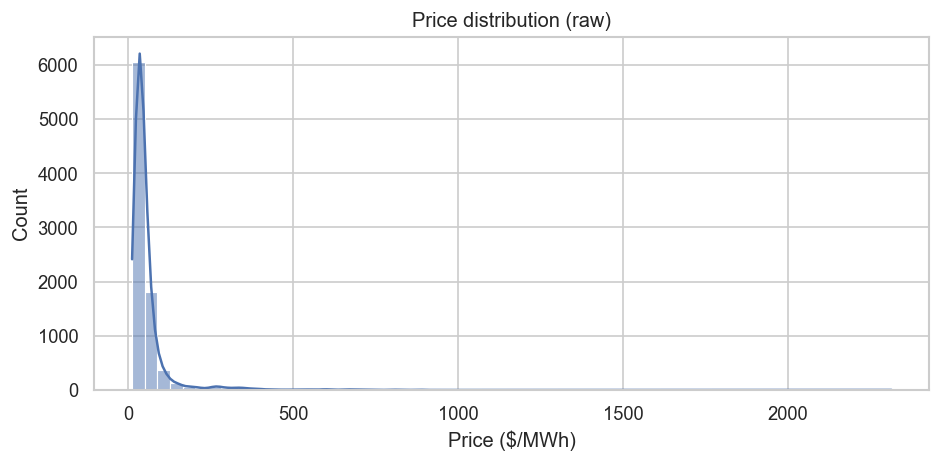
\includegraphics[width=0.75\linewidth]{../plots/eda_price_distribution.png}
  \caption{Target price distribution}
  \label{fig:appendix-price-distribution}
\end{figure}

\begin{figure}[!htbp]
  \centering
  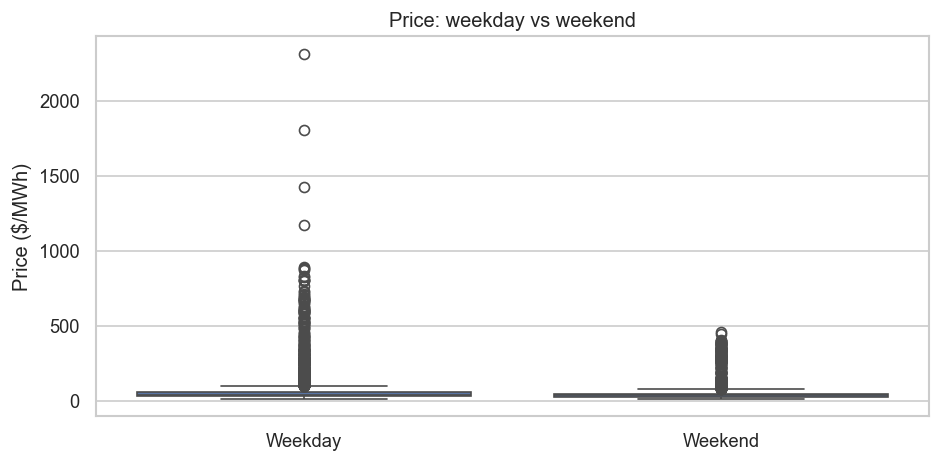
\includegraphics[width=0.75\linewidth]{../plots/eda_weekday_vs_weekend.png}
  \caption{Weekday and weekend price comparison}
  \label{fig:appendix-weekday-weekend}
\end{figure}

\begin{figure}[!htbp]
  \centering
  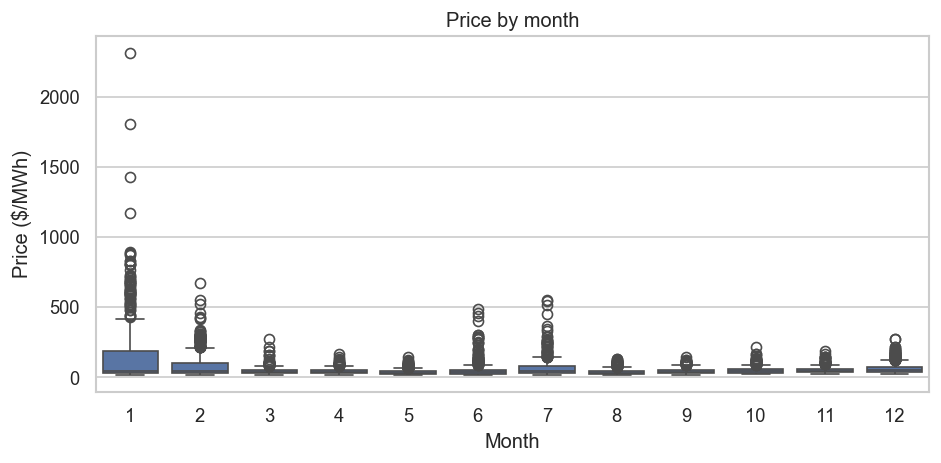
\includegraphics[width=0.75\linewidth]{../plots/eda_price_by_month.png}
  \caption{Monthly price variation}
  \label{fig:appendix-price-by-month}
\end{figure}

\begin{figure}[!htbp]
  \centering
  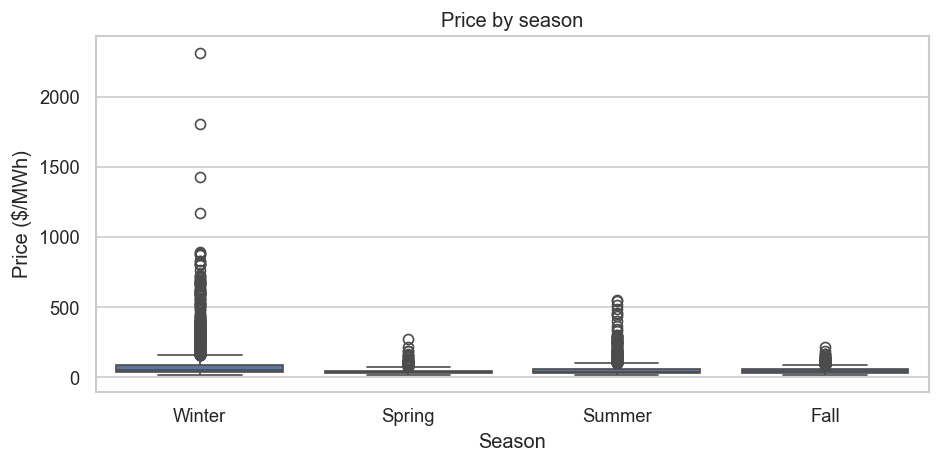
\includegraphics[width=0.75\linewidth]{../plots/eda_price_by_season.png}
  \caption{Seasonal price variation}
  \label{fig:appendix-price-by-season}
\end{figure}

\begin{figure}[!htbp]
  \centering
  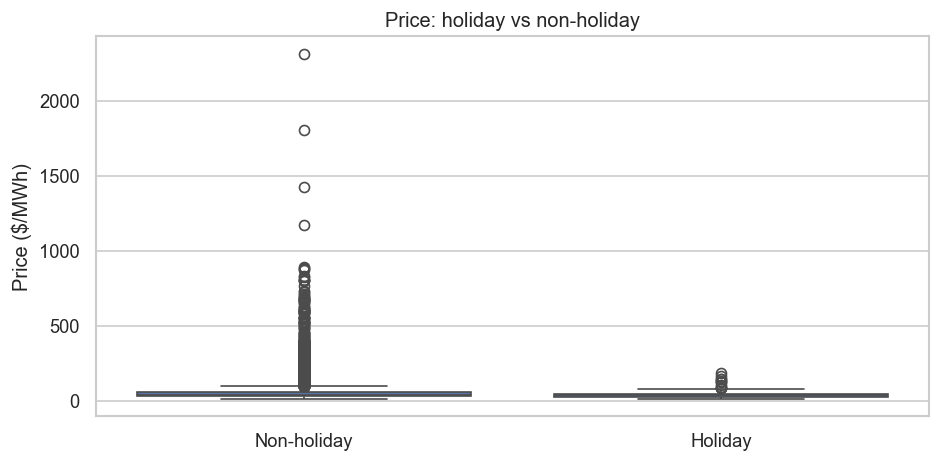
\includegraphics[width=0.75\linewidth]{../plots/eda_holiday_vs_non_holiday.png}
  \caption{Holiday and non-holiday price comparison}
  \label{fig:appendix-holiday}
\end{figure}

\end{document}
